\chapter{Tensoren}
\label{h:tensoren}
In dit hoofdstuk gaan we het hebben over de notatie-conventies en over tensoren. We zullen enkel de aspecten aanraken die noodzakelijk zijn om rest van deze tekst te kunnen begrijpen.

In de vakliteratuur vormt men tensoren om naar matrices en vectoren. Vervolgens werkt men dan verder met deze matrices en vectoren. Wij gaan in deze tekst niet met matrices of vectoren werken maar wel rechtstreeks met de elementen van de tensoren. 

%\todo{intro + vermelden parafrazering + misschien titel CPD noemen}

\section{Notaties}
In deze tekst gebruiken we volgende notatie-conventies:

\begin{tabular}{l l l}
    Vector						& Vetgedrukte kleine letters					& $\vect{v}$\\
    Matrix 						& Normale hoofdletters							& $M$\\
    Tensor 						& Hoofdletters in een kalligrafisch geschrift	& \TT\\
    Element						& Kleine letters met een index in subscript	& $e_i$\\
\end{tabular}

Merk op dat de index ook een tupel kan zijn. Deze tupel is dan vet gedrukt in kleine letters. Een voorbeeld: $t_{\ii}$.

We gebruiken ook verzamelingen van matrices. Deze verzamelingen worden genoteerd in vetgedrukte hoofdletters. Een voorbeeld: \UUU{}. De i-de matrix van de verzameling \UUU{} noteren we als \UU{i}.

\section{Tensoren}
Men kan een tensor voorstellen als een $N$-dimensionale rij. We spreken dan over een $N$-de-orde tensor $\tensor{T}$. $\tensor{T}$ heeft $N$ modes en orde is gelijk aan $N$. Formeel schrijven we $\tensor{T} \in \R^{I_1 \times \dotsb \times I_N}$. $I_n$ is gelijk aan het aantal elementen in mode $n$. Tensoren zijn ook gedefini\"eerd voor complexe getallen, maar we gaan ons beperken tot de re\"ele getallen.

Een element van een derde-orde tensor $\tensor{T}$ noteren we als $t_{ijk}$. $i$ komt overeen met de eerste mode, $j$ met de tweede en $k$ met de derde mode. Een element van een $N$-de-orde tensor schrijven we als $t_{\ii{}}$ met $\ii{} \in \I$. We defini\"eren de indexverzameling $\I$ als de verzameling van alle tupels die een geldige index van de tensor zijn.
\[
    \I = \{\ii{} \in \N_0^N | \forall n \in [1, N]: i_n \in [1, I_n]\}
\]

%\todo{Vergelijking met matrix en eventueel vector}
%\todo{Is het correct om te zeggen dat een matrix een tweede-orde tensor is? En omgekeerd?}

Er bestaan ook tweede -en eerste-orde tensoren. Een tweede-orde tensor is gekend onder de naam matrix. Een eerste-orde matrix noemen we ook een vector. We zullen steeds de matrix (vector)-notatie gebruiken wanneer een tensor van de tweede(eerste) orde is.

We kunnen tensoren met elkaar opgetellen. $\tens{A} + \tens{B} = \tens{C}$ als en slechts als:
\[
	\forall \ii{} \in \I: c_{\ii{}} = a_{\ii{}} + b_{\ii{}}
\]

Het is ook mogelijk om de Frobeniusnorm te nemen van een tensor. Deze norm is gelijk aan de som van de kwadraten van de elementen van de tensor. Wanneer we in deze tekst over de norm van een tensor spreken, spreken we over de Frobeniusnorm.
\[
	||\tens{T}||^2 = \sum_{\ii{} \in \I} t_{\ii{}}^2
\]

\section{Canonieke Polyadische Decompositie (CPD)}
We kunnen een tensor $\tens{T}$ benaderen met de Canonieke Polyadische Decompositie, afgekort CPD. %\todo{referentie}
Deze ontbinden kunnen we als volgt defini\"eren:
\[
    t_{\ii{}} \approx c_{\ii{}} = \sum_{r=1}^{R} \prod_{n=1}^{N} u^{(n)}_{i_{n}r} \qquad
    \text{met $\ii{} \in \I$, $R \in \N_0$ en $\mUU{n} \in \R^{I_n \times R} $}
\]
We noemen R de rang van de decompositie en \UUU{} noemen we de factormatrices. Zie figuur \ref{cpdTekening} voor een visuele voorstelling van de CPD van een derde-orde tensor.

\begin{figure}
\centering
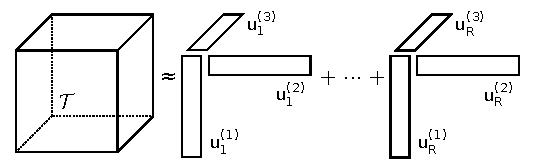
\includegraphics{cpd}
\caption{\label{cpdTekening}Een visuele voorstelling van de CPD van een derde-orde tensor. Bron: \cite[p.~4]{laurent}}
\end{figure}

%\todo{Tekening, nog wat uitleg + toepassingen}
%\todo{Naam voor 'u' opzoeken of verzinnen. Misschien factormatrix ofzo}
%\todo{Dat ding van de rank waarbij een tensor 50proc kans benadering exact is.}

\section{Gradi\"ent gebaseerde optimalisatie-algoritmes}
\label{h:algo} 

\TT{} is slechts een benadering voor \CC{}. Er zijn veel algoritmes om de factormatrices te vinden zodat \CC{}, \TT{} zo best mogelijk benadert. We defini\"eren de residu-tensor \FF{} als volgt:
\begin{align*}
    \tens{F} &= \tens{C} - \tens{T}\\
    f_{\ii{}} &= \left( \sum_{r=1}^{R} \prod_{n=1}^{N} u^{(n)}_{i_{n}r} \right) - t_{\ii{}} \qquad \text{met $\ii{} \in \I$}\\
\end{align*}

We defini\"eren de doelfunctie $f(\T, \mUUU)$ als de frobeniusnorm van \FF{}. Wanneer we $f$ schrijven bedoelen we %soms ook
de waarde van $f(\T, \mUUU)$ voor de huidige waardes van \TT{} en \UUU{}.
\begin{align*}
    f(\T, \mUUU) &= ||\tens{F}||^2\\
    f(\T, \mUUU) &= \sum_{\ii{} \in \I} f_{\ii{}}^2\\
    f(\T, \mUUU) &=  \sum_{\ii{} \in \I} \left( \left( \sum_{r=1}^{R} \prod_{n=1}^{N} u^{(n)}_{i_{n}r} \right) - t_{\ii{}} \right)^2
\end{align*}

Het doel van elk optimalisatie-algoritme is om de \UUU{} te vinden voor een gegeven \TT{} waarvoor $f(\T, \mUUU)$ minimaal is.
\[
    \min_{\mUUU} \sum_{\ii{} \in \I} \left( \left( \sum_{r=1}^{R} \prod_{n=1}^{N} u^{(n)}_{i_{n}r} \right) - t_{\ii{}} \right)^2
\]

De gradi\"ent gebaseerde optimalisatie-algoritmes vormen een groep van algoritmes om een optimale \UUU{} te vinden. E\'en van de eenvoudigste algoritmes in deze groep is de methode van de stijlste helling maar er zijn ook geavanceerdere algoritmes zoals beperkt-geheugen BFGS \cite{bfgs}. Wat al deze algoritmes gemeenschappelijk hebben is dat ze de gradi\"ent van $f(\T, \mUUU)$ gebruiken om op een iteratieve manier tot een optimale oplossing te komen.

We stellen de gradi\"enten voor als matrices, de gradi\"entmatrices \GGG{}. \GGG{} heeft dezelfde dimensies als \UUU{}. We gaan nu afleiden hoe men de gradi\"ent van $f(\T, \mUUU)$ berekent. Aan de linkerkant gaan we de gradi\"ent afleiden van een derde-orde tensor voor een element uit de eerste gradi\"entmatrix. Aan de rechterkant gaan we de gradi\"ent afleiden van tensoren in het algemeen.
\begin{align*}
	g^{(1)}_{ir} 	&:= \frac{\partial f(\T, \mUUU)}{\partial u^{(1)}_{ir}} &
    g^{(n)}_{ir} 	&:= \frac{\partial f(\T, \mUUU)}{\partial u^{(n)}_{ir}}\\
%    
					&=\frac{\partial}{\partial u^{(1)}_{ir}} \frac{1}{2}\sum_{i'}^{I_1}\sum_{j'}^{I_2}\sum_{k'}^{I_3}\left(c_{i'j'k'} - t_{i'j'k'} \right)^2 &
					&=\frac{\partial}{\partial u^{(n)}_{ir}} \frac{1}{2}\sum_{\iii{} \in \I}\left(c_{\iii{}} - t_{\iii{}} \right)^2\\
%					
					&= \frac{1}{2} \sum_{j'}^{I_2}\sum_{k'}^{I_3} \frac{\partial}{\partial u^{(1)}_{ir}} \left(c_{ij'k'} - t_{ij'k'} \right)^2 &
					&= \frac{1}{2} \sum_{\substack{\iii{} \in \I\\ i'_n = i}} \frac{\partial}{\partial u^{(n)}_{ir}} \left(c_{\iii{}} - t_{\iii{}} \right)^2\\
%					
					&= \frac{1}{2} \sum_{j'}^{I_2}\sum_{k'}^{I_3} 2 \left(c_{ij'k'} - t_{ij'k'} \right) \frac{\partial c_{ij'k'}}{\partial u^{(1)}_{ir}} &
					&= \frac{1}{2} \sum_{\substack{\iii{} \in \I\\ i'_n = i}} 2 \left(c_{\iii{}} - t_{\iii{}} \right) \frac{\partial c_{\iii{}}}{\partial u^{(n)}_{ir}}\\
%					
					&=\sum_{j'}^{I_2}\sum_{k'}^{I_3} f_{ij'k'} \frac{\partial}{\partial u^{(1)}_{ir}} \sum_{r'=1}^{R}  u^{(1)}_{ir'} u^{(2)}_{j'r'} u^{(3)}_{k'r'}&
					&=\sum_{\substack{\iii{} \in \I\\ i'_n = i}} f_{\iii{}} \frac{\partial}{\partial u^{(n)}_{ir}} \sum_{r'=1}^{R} \prod_{n'=1}^{N} u^{(n')}_{i'_{n'}r'}\\
%					
	g^{(1)}_{ir}	&=\sum_{j'}^{I_2}\sum_{k'}^{I_3} f_{ij'k'} u^{(2)}_{j'r} u^{(3)}_{k'r}&
	g^{(n)}_{ir}	&=\sum_{\substack{\iii{} \in \I\\ i'_n = i}} f_{\iii{}} \prod_{\substack{n'=1\\n'\neq n}}^{N} u^{(n')}_{i'_{n'}r}
\end{align*}